%************************************************
\section{The API} % (fold)
\label{sec:impl_api}
%************************************************
In Section \ref{sec:api} we have designed a RESTful API serving JSON content for third party service to retrieve the egocentric context data in the SSM Sets. There are many ways one can implement a RESTful API in Java, ranging from using one of the many existing libraries, to building it from scratch. The EgoSim project is a simple Java application with no server-side capabilities. Meaning that in order to provide an API we would first need to create a HTTP server to intercept and parse the requests, with capabilities to serve multiple requests at the same time.\\

Building up the API from scratch, would have been a redundant work given a wide range of third party libraries offering these features ready made. One of these frameworks is Restlet\footnote{\url{http://restlet.com}}. We have chosen Restlet, as it is one of the leading open source RESTful web API frameworks for Java. Moreover, we have already worked with it in previous projects, saving us time when integrating the library into our framework.\\

The classes that implement the functionality of our API are depicted in Figure \ref{fig:impl_api}. The ContextApiServer is initialized in the monitoring service component \ref{sec:impl_monitoring_service}. This starts up a HTTP server accessible within the network the physical computer is connected to. If accessed from the same computer the simulator is running on, it can be accessed on \url{http://localhost:8182/context/api}. This endpoint accepts only GET requests, each request being handled by a new instance of the ApiContextResource class.
\begin{figure}[H]
	\centering
	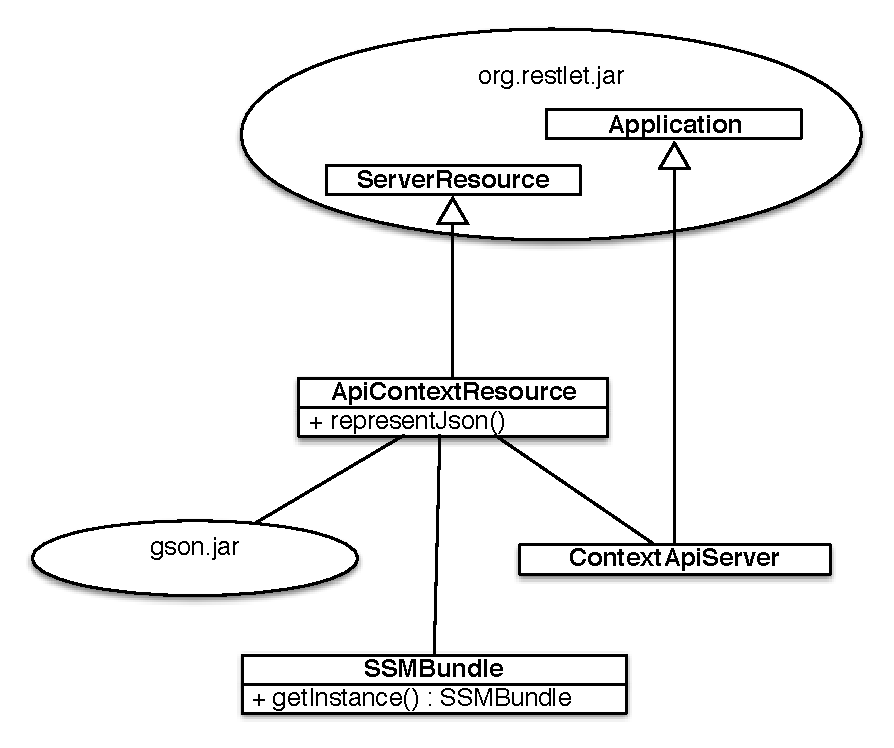
\includegraphics[width=\linewidth]{gfx/Chapter4/api}
	\caption{Class Diagram of the API classes and their third party dependencies}
	\label{fig:impl_api}
\end{figure}

The endpoint accepts an URL parameter called \emph{name} to specify the name of the set the third party service wants to retrieve. The possible values are: \emph{worldSpace}, \emph{perceptionSpace}, \emph{recognizableSet}, \emph{examinableSet}, \emph{actionSpace}, \emph{selectedSet}, \emph{manipulatedSet} and \emph{all}. For example, to access the content of the World Space, the third party service would issues the following GET request:\\
\url{http://localhost:8182/context/api?name=worldSpace}.\\

Whenever a new request is encountered, the ApiContextResource retrieves the data from the requested sets and serializes them to the JSON format. To convert the set contents to JSON we have used the GSON\footnote{\url{https://code.google.com/p/google-gson/}} library, a Java library that can be used to convert Java Objects into their JSON representation. An example JSON output of the World Space from the API is illustrated in Figure \ref{fig:impl_json_example}.
\begin{figure}[H]
	\centering
	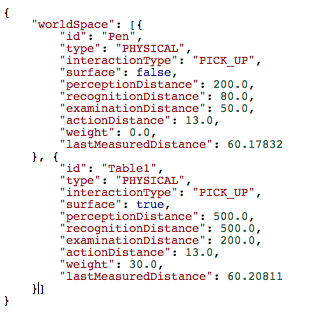
\includegraphics[width=\linewidth]{gfx/Chapter4/json_example}
	\caption{JSON output example}
	\label{fig:impl_json_example}
\end{figure}
% section impl_api (end)